%==================================================
%      PREAMBOLO e DICHIARAZIONI INIZIALI
%==================================================
\documentclass[10pt,oneside,a4paper]{article}

\usepackage[latin1]{inputenc} 
\usepackage[italian]{babel}
\usepackage[T1]{fontenc}
\usepackage{siunitx} %Inserisce automaticamente i dati con le unit�  di misura correttamente formattate del SI (utilizzo: \SI{0.82}{m^2}, in generale \SI{misura con il punto decimale}{unit�  di misura})
\sisetup{output-decimal-marker = {.}, separate-uncertainty = true, input-uncertainty-signs = \pm, detect-weight=true, detect-family=true} %per usare SI con il punto decimale
\usepackage{listings} %Per citare codice informatico formattandolo correttamente
\usepackage{amsmath,amsthm,verbatim,amssymb,amsfonts,amscd,graphicx,mathtools}
\usepackage[makeroom]{cancel}
\newcommand{\abs}[1]{\left\lvert\,#1\,\right\rvert}
\usepackage{geometry}
\usepackage{epigraph}
\usepackage{booktabs}	%tabelle migliorate
\usepackage{tablefootnote}	%note a pi� di pagina in tabella
\usepackage{threeparttable} %tabella con note a pi� di tabella
\usepackage{caption}	%descrizione per figure
\usepackage{dblfnote}
\captionsetup{tableposition=top,figureposition=bottom,font=small} %setup descrizione
\usepackage{float}
\usepackage{esvect} %vettori
\usepackage{longtable} %tabelle lunghe
\usepackage[dvipsnames]{xcolor}
\definecolor{sepia}{HTML}{80002A}
\usepackage[colorlinks=true, citecolor=black, linkcolor=sepia, urlcolor=black]{hyperref}
\usepackage{mathrsfs}
\usepackage{circuitikz}
\ctikzset{bipoles/resistor/height=0.2}
\ctikzset{bipoles/resistor/width=0.4}
\usepackage{enumitem} %Liste senza spazi verticali
\setlist{noitemsep}
\usepackage{amsmath}

\interfootnotelinepenalty=10000


\usepackage{multicol}
\newenvironment{Figure}
  {\par\medskip\noindent\minipage{\linewidth}}
  {\endminipage\par\medskip}

\newcommand{\var}{\operatorname{var}}
\newcommand{\cov}{\operatorname{cov}}


\usepackage{listings} %Per inserire codice
\lstnewenvironment{codice_c}[1][]
{\lstset{basicstyle=\small\ttfamily, columns=fullflexible,
keywordstyle=\color{red}\bfseries, commentstyle=\color{blue},
language=C, basicstyle=\small,
numbers=left, numberstyle=\tiny,
stepnumber=2, numbersep=5pt, frame=shadowbox,  showstringspaces=false, #1}}{}

%==================================================
%                  PRIMA PAGINA
%==================================================

\title{\textsc{\textbf{Esercitazione 5}: Amplificatore operazionale 3}}
\author{\small{G. Galbato Muscio} \and \small{L. Gravina} \and \small{L. Graziotto}}
\date{20 Novembre 2018}

\begin{document}
	\begin{figure}
		\centering
		
\includegraphics[scale=0.5, trim={2.8cm 8.9cm 0 9cm}, clip]{logo.png}
	\end{figure}
	\maketitle
	\begin{center} 
		\fbox{{\fontsize{12pt}{8mm}\textsc{Gruppo 11}}} \\
	\end{center}
\hrule
\vspace{0.5cm}
\renewcommand{\abstractname}{Abstract}
\begin{abstract}
Si realizzano un filtro VCVS passa basso utilizzando un OP-AMP LM358N e un generatore di rumore bianco basato su transistor di tipo 2N2222A; si studia l'andamento del modulo e della fase della funzione di trasferimento del filtro passa basso al variare della frequenza del segnale in ingresso.
\end{abstract}
\vspace{4cm}
\tableofcontents %Indice
\newpage


\pagebreak
\begin{multicols}{2}
%==================================================
%      		FILTRO VCVS
%==================================================
\section{Filtro VCVS passa basso}
Si utilizza nel seguito l'amplificatore operazionale LM358N, e lo si alimenta con una differenza di potenziale di $\pm \SI{15}{V}$, connettendo gli ingressi \texttt{V+} e \texttt{GND} alla doppia alimentazione in continua, positiva e negativa. 

Si realizza il seguente filtro passa basso VCVS.

%ESEMPIO DI CIRCUITO
\begin{center}
\begin{circuitikz}[scale=0.7]
\draw (0,0) node[op amp, yscale=-1] (opamp) {}
(opamp.+) -- ++(-1.2,0) node[circ]{} to[C=$C_1$] ++(0,-1.5) node[ground]{}
(opamp.out) to[short, *-*] ++(0.5,0) node[right] {$v_\text{o}$}
(opamp.-) -- ++(0,-1) node[circ] {} to[R=$R_4$] ++(0,-1.5) node[ground]{}
(opamp.-) ++(0,-1) to[R=$R_3$] ++(3.4,0) -| (opamp.out)
(opamp.+) ++(-1.2,0) to[R=$R_2$] ++(-2,0) to[R=$R_1$] ++(-2,0) node[circ]{} node[left]{$v_i$}
(opamp.+) ++(-1.2,0) ++(-2,0) node[circ]{} -- ++(0,1.5) to[C=$C_2$] ++(4,0) -| (opamp.out)
;\end{circuitikz}
\end{center}

Nell'ipotesi di amplificatore ideale (quindi corrente d'ingresso nulla e tensioni ai due ingressi uguali) la funzione di trasferimento assume la forma 
\begin{equation}\label{eq:trasferimento} %IL PRIMO MODO PER RIPORTARE UN'EQUAZIONE LUNGA � SPEZZARLA
\begin{aligned}
	\text{T}(\omega) =& k\big[1- \omega^2 R_1 R_2  C_1 C_2 + \\
	&\;+ j \omega^2(C_1(R_1 + R_2) + R_1 C_2 (1-k))\big]^{-1}
\end{aligned}
\end{equation}
\normalsize
che per $R_2 = R_1$ e $C_2 = C_1$ si semplifica in
\begin{equation}\label{eq:trasferimento_approx}
	\text{T}(\omega) = \frac{k}{1 - (\omega R_1 C_1)^2 + j \omega R_1 C_1 (3-k)}
\end{equation}
Nel caso generale, modulo e fase della funzione di trasferimento sono rispettivamente
\begin{equation}\label{eq:modulo_trasf}%IL SECONDO MODO � SCALARLA
\begin{aligned}
	\vert \text{T} (\omega) \vert &= k\bigg[\left( 1 - R_1 R_2 \omega^2 C_1 C_2 \right)^2 + \\
	&+ \omega^2 \left(C_1 (R_1 + R_2) + R_1 C_2 (1-k)\right)^2\bigg]^{-\frac{1}{2}}
\end{aligned}
\end{equation}
\small{
\begin{equation}\label{eq:fase_trasf}
	\phi(\omega) = \text{arctan}\left(\frac{\omega(C_1(R_1+R_2)+R_2C_2(1-k))}{1-R_1R_2\omega^2C_1C_2}\right)
\end{equation}}
\normalsize
%Il modulo e la fase della funzione di trasferimento valgono dunque
%\small{
%\[
%\lvert T(w)\rvert = \frac{k}{\big(1-\omega^2(C_1R_1)^2\big)^2+\big((3-k)^2\omega^2C_1^2R_1^2\big)^2}
%\]}
%\small{
%\[
%\phi(\omega)= -\arctan\left(\frac{(3-k)\omega C_1R_1}{1-\omega^2(C_1R_1)^2}\right)
%\]}
%\normalsize


Si vuole scegliere una resistenza $R_1$ sufficientemente grande (dell'ordine delle decine di \SI{}{\kilo\ohm}) per aumentare la resistenza di ingresso $R_\text{i}$ del filtro e dunque ridurre le perturbazioni del segnale in ingresso.

Per ottenere $R_1$ il pi� possibile simile a $R_2$ si � usato per la seconda un trimmer; un altro trimmer � stato usato per la resistenza $R_3$ in modo da poter controllare con precisione il valore di amplificazione del filtro.

Il circuito � stato realizzato con i seguenti componenti fissi:
\begin{itemize} %Lo spazio verticale � stato tolto con \setlist{noitemsep} nell'header, rimuovere quella riga per avere una lista classica
	\item[--] $R_1 = \SI{8.22 \pm 0.04}{\kilo\ohm}$;
	\item[--] $R_2 = \SI{8.21 \pm 0.04}{\kilo\ohm}$;
	\item[--] $R_4 = \SI{4.65 \pm 0.02}{\kilo\ohm}$;
	\item[--] $C_1 = \SI{20.79 \pm 0.02}{\nano\farad}$;
	\item[--] $C_2 = \SI{20.80 \pm 0.02}{\nano\farad}$
\end{itemize}
Il valore di $R_3$ non � presente tra gli altri non avendo esso un valore fisso, e sar� riportato nel seguito.

Si stima la frequenza di taglio del circuito, dati i componenti usati, dalla~(\ref{eq:trasferimento}):
\[
f_T = \frac{1}{2\pi\sqrt{R_1R_2C_1C_2}} = \SI{932 \pm 9}{Hz}.
\]

\subsection{Overshooting}

Come prima misura, si sceglie il valore di 
\[
R_3 = (k-1) R_4 = \SI{6.98 \pm 0.03}{\kilo\ohm},
\] ovvero si sceglie $k = \SI{2.5}{}$: essendo $k > k_\text{limite} \equiv 1.586$ ci si aspetta un picco del modulo della funzione di trasferimento in corrispondenza della frequenza di taglio del filtro. 

I risultati delle misure sono riportati in Tabella~\ref{tab:filtro_uno}, in Appendice. Dalle misure di tensione a frequenze sufficientemente basse (si considerano le prime $9$ misure) si pu� ricavare un valore di amplificazione reale pari a $A_v = \SI{2.54 \pm 0.08}{}$ con incertezza data dalla deviazione standard; il valore misurato risulta compatibile con quello previsto, ossia $A_v^\text{(atteso)} = k$. Gli andamenti del modulo e della fase della funzione di trasferimento sono riportati in Figura~\ref{fig:modulo_filtro} e in Figura~\ref{fig:fase_filtro}, con sovrapposte ai dati sperimentali le curve teoriche ottenute da (\ref{eq:modulo_trasf}) e (\ref{eq:fase_trasf}) corrispondenti ai valori misurati dei componenti.


Gli andamenti sono compatibili con quelli teorici: il modulo ha un massimo in corrispondenza di $f_T = \SI{901 \pm 45}{\hertz}$, valore che � stato stimato come la frequenza intermedia tra le misure corrispondenti ai due valori di ${\vert T(f=\omega/2\pi) \vert}$ pi� elevati, compatibile con quello ricavabile da (\ref{eq:trasferimento_approx}) pari a $f_T^{\text{(attesa)}} = \SI{932 \pm 9}{\hertz}$; inoltre la fase assume il valore di $-\pi / 2$ in corrispondenza di $f_\phi = \SI{916 \pm 52}{\hertz}$ inferito dalla retta congiungente i due punti sperimentali pi� vicini al valore teorico assunto della fase alla frequenza di taglio, anche questo valore risulta compatibile con quello teorico.

Interpolando linearmente la regione decrescente si ottiene una pendenza di \SI{-41 \pm 2}{\dB / dec}, coerente con quanto previsto per il filtro VCVS.

\subsection{Butterworth}

Come seconda misura si sceglie il valore di $R_3 = \SI{2.74 \pm 0.01}{\kilo\ohm}$, ovvero si sceglie $k = \SI{1.589} \approx \,k_\text{limite}$, cio� si realizza un filtro \emph{Butterworth}. In queste condizioni non ci si aspetta alcun picco del modulo della funzione di trasferimento. I risultati delle misure sono riportati in Tabella~\ref{tab:filtro_due} in Appendice, gli andamenti del modulo e della fase della funzione di trasferimento sono riportati in Figura~\ref{fig:modulo_filtro} e in Figura~\ref{fig:fase_filtro}.

Gli andamenti sono compatibili con quelli teorici. Dalle prime $7$ misure si ottiene una stima di $A_v = \SI{1.57 \pm 0.02}{}$, compatibile con il valore previsto di $A_v^\text{(atteso)} = k$. Dall'andamento del modulo si stima una frequenza di taglio pari a $f_T = \SI{977 \pm 44}{\hertz}$, ottenuta come la frequenza dell'intersezione tra l'interpolazione lineare in regime costante (misure da 1 a 7) traslata verso il basso di $\SI{-3}{\decibel}$\footnote{Ossia il valore del modulo della funzione di trasferimento alla frequenza di taglio.} e quella a regime di discesa asintotica (misure da 9 a 20), valore compatibile con quello teorico di $f_T^{\text{(attesa)}} = \SI{932 \pm 9}{\hertz}$; anche dall'andamento della fase si pu� stimare, come fatto nel paragrafo precedente, la frequenza di taglio ottenendo $f_\phi = \SI{919 \pm 53}{\hertz}$ ancora compatibile con il valore previsto, dati i componenti. L'interpolazione lineare della regione decrescente, inoltre, fornisce una pendenza di \SI{-33.9 \pm 0.8}{\dB / dec}, coerente con quanto previsto per il filtro del secondo ordine. Si osserva inoltre che la pendenza per il \emph{Butterworth} � inferiore a quella del filtro in modalit� \emph{Overshooting}. Si riporta in Tabella~\ref{tab:riepilogo} un confronto tra valori previsti e ottenuti per il filtro VCVS in entrambe le modalit�.

\begin{table*}
\captionof{table}{Riepilogo dei valori teorici e stimati per il filtro VCVS}
\label{tab:riepilogo}
\begin{center}
\begin{tabular}{c|c|c}
 									& \emph{Overshooting} & \emph{Butterworth} \\
\hline 
$k$  								&	\SI{2.5}{}			&		\SI{1.589}{}			\\
$A_v$								& \SI{2.54 \pm 0.08}{} & \SI{1.57 \pm 0.02}{} \\
$f_T^{\text{(attesa)}}$ [\SI{}{\hertz}]	& \SI{932 \pm 9}{} 	& \SI{932 \pm 9}{} \\
$f_T^{\text{(modulo)}}$ [\SI{}{\hertz}]	& \SI{901 \pm 45}{} & \SI{977 \pm 44}{} \\
$f_\phi$ [\SI{}{\hertz}]				& \SI{916 \pm 52}{} & \SI{919 \pm 53}{} \\
Pendenza [\SI{}{\dB / dec}]			& \SI{-41 \pm 2}{}  & \SI{-33.9 \pm 0.8}{} \\
\hline
\end{tabular}
\end{center}
\end{table*}

\begin{Figure}
	\begin{center}
	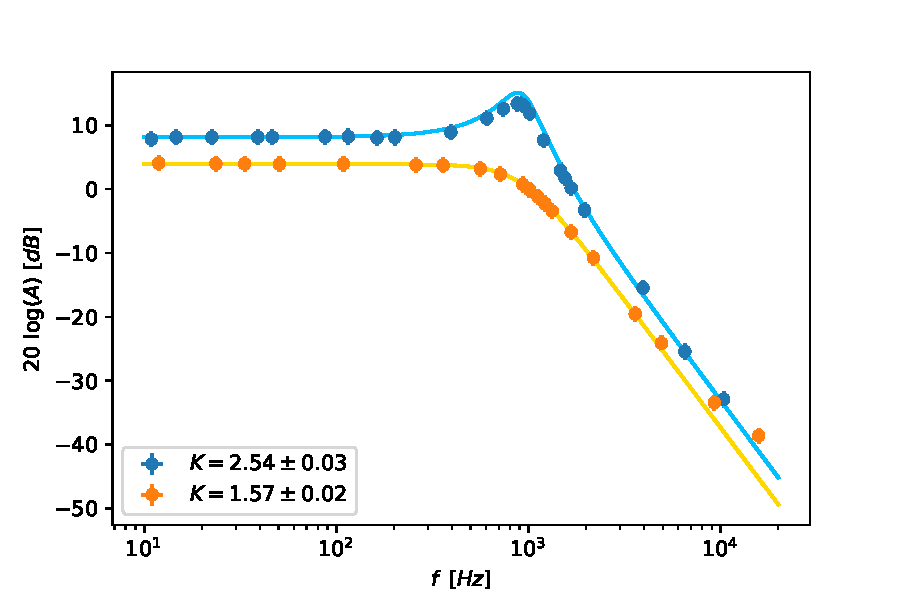
\includegraphics[width=\linewidth]{double_abs.pdf}
	\captionof{figure}{Diagramma di Bode del modulo della funzione di trasferimento al variare delle frequenze}
	\label{fig:modulo_filtro}
	\end{center}
\end{Figure}

\begin{Figure}
	\begin{center}
	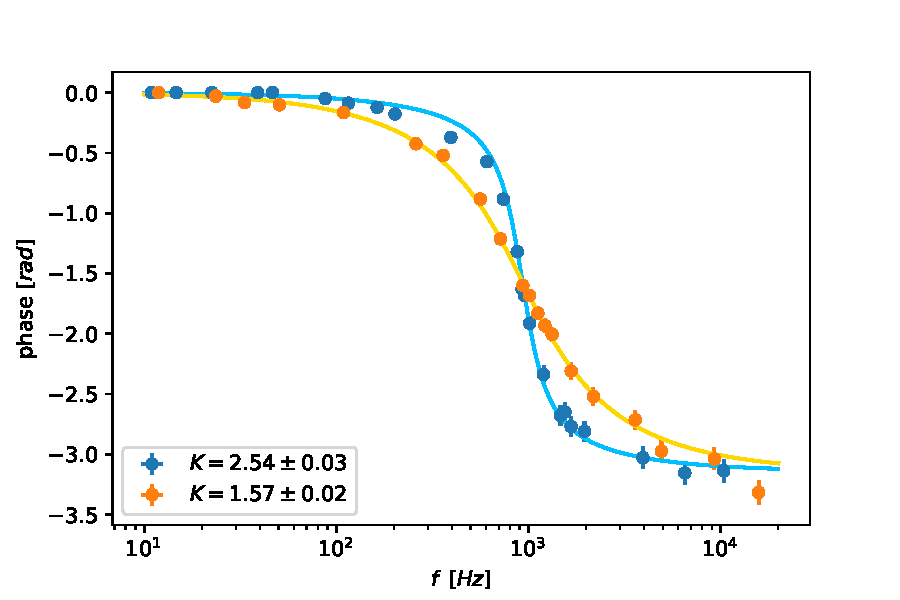
\includegraphics[width=\linewidth]{double_phi.pdf}
	\captionof{figure}{Diagramma di Bode della fase della funzione di trasferimento al variare delle frequenze}
	\label{fig:fase_filtro}
	\end{center}
\end{Figure}

\pagebreak

%==================================================
%      		GENERATORE DI RUMORE
%==================================================
\section{Generatore di rumore}
Si realizza un generatore di rumore \emph{bianco} amplificando quello generato da una giunzione \texttt{pn} in regime di breakdown; il circuito costruito � il seguente,
\begin{center}
\begin{circuitikz}[scale=0.9]
\draw (0,0) node[npn, xscale=-1, yscale=-1] (Q1) {}
(Q1) node[left]{$Q_1$}
(Q1.E) to[R=$R_1$] ++(0,1.5) node[circ] (top) {} to[short, -*] ++(0,0.5) node[above]{$V_\text{in}$}
(Q1.E) node[circ]{} -- ++(-1.3,0) to[C=$C_1$] ++(0,1.5) -| (top)
(2.5,0) node[npn] (Q2) {}
(Q2) node[]{$Q_2$}
(Q2.B) to[short] (Q1.B)
(top) -- ++(2.5,0) to[R=$R_2$] (Q2.C)
(Q2.C) node[circ]{} to[C] ++(2,0) node[circ] (bottom) {}-- ++(0.3,0) node[circ]{} node[right]{$V_o$}
(Q2.C) ++(1,-0.5) node[below]{$C_2$}
(bottom) to[R=$R_3$] ++(0,-1.1) node[ground]{}
(Q2.E) node[circ]{} to[R=$R_4$] ++(0,-1.3) 
(Q2.E) -- ++(1.3,0) to[C=$C_3$] ++(0,-1.3) to[short] ++(-1.3,0) ++(0.7,0) node[ground]{} 
;\end{circuitikz}
\end{center}
dove i componenti scelti hanno valori (misurati con multimetro e ponte):
\begin{itemize} %Lo spazio verticale � stato tolto con \setlist{noitemsep} nell'header, rimuovere quella riga per avere una lista classica
	\item[--] $\text{V}_\text{in} = \SI{12.0 \pm 0.4}{\volt}$;
	\item[--] $R_1 = \SI{0.692 \pm 0.003}{\mega\ohm}$;
	\item[--] $R_2 = \SI{4.68 \pm 0.02}{\kilo\ohm}$;
	\item[--] $R_3 = \SI{97.5 \pm 0.5}{\kilo\ohm}$;
	\item[--] $R_4 = \SI{1.001 \pm 0.005}{\kilo\ohm}$;
	\item[--] $C_1 = \SI{98.6 \pm 0.1}{\nano\farad}$;
	\item[--] $C_2 = \SI{8.647 \pm 0.004}{\micro\farad}$
	\item[--] $C_3 = \SI{8.758 \pm 0.004}{\micro\farad}$
\end{itemize}

L'alimentazione $V_\text{in}$ � fornita con un generatore di tensione; poich� tale alimentazione sar� in comune con il filtro, anch'esso verr� alimentato con una differenza di potenziale di $\pm \SI{12}{V}$.
Il collettore del transistor $\text{Q}_1$ � lasciato flottante in quanto lo si vuole utilizzare come diodo; entrambi i transistor sono di tipo 2N2222A.

Si riporta in Figura~\ref{fig:rumore} il segnale di rumore rilevato dall'oscilloscopio, il rumore ha ampiezza quadratica media misurata con l'oscilloscopio pari a $\text{V}_\text{noise} \simeq \SI{117}{\milli\volt}$: non si � in grado di fornire un'incertezza per questa stima, in quanto il valore indicato dall'oscilloscopio, anche aumentando la scala temporale della visualizzazione, non � stabile, bens� varia imprevedibilmente in un range dell'ordine di $10^2$ \SI{}{mV}.

\begin{Figure}
	\begin{center}
	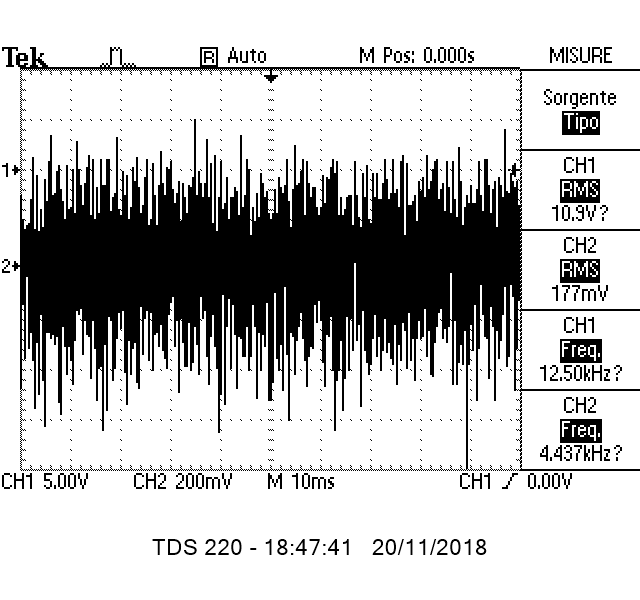
\includegraphics[width=0.9\linewidth]{noise.PNG}
	\captionof{figure}{Screenshot del segnale di rumore bianco}
	\label{fig:rumore}
	\end{center}
\end{Figure}

Collegando l'uscita del generatore all'ingresso del filtro passa basso costruito alla sezione precedente si ottiene il segnale riportato in Figura~\ref{fig:rumore_filtro} (al \texttt{CH1} dell'oscilloscopio � collegata l'uscita del filtro VCVS, mentre al \texttt{CH2} l'uscita del generatore di rumore): questo rumore risulta attutito rispetto al caso precedente, in quanto le componenti a frequenza pi� alta vengono abbattute dal filtro; si confrontino infatti i due andamenti, che per maggiore chiarezza sono riportati alla stessa scala. Possiamo nuovamente misurare l'ampiezza quadratica media, ottenendo $\text{V}_\text{noise} \simeq \SI{22}{\milli\volt}$, tenendo conto delle stesse problematiche della misura esposte in precedenza. � visibile infatti in questo caso un valore RMS del rumore pari a circa \SI{260}{mV}, dunque si pu� dedurre che il filtro agisca riducendo di un fattore $10$ l'ampiezza quadratica media del segnale di \emph{noise} in ingresso.


\begin{Figure}
	\begin{center}
	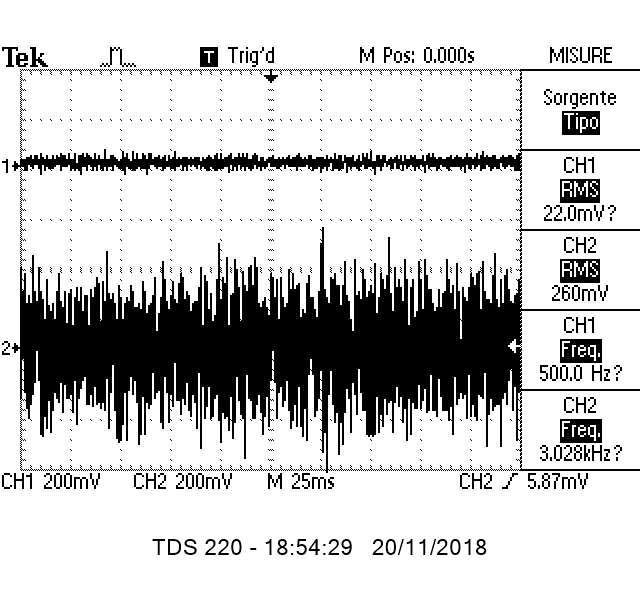
\includegraphics[width=0.9\linewidth]{filtered_noise.PNG}
	\captionof{figure}{Screenshot del segnale di rumore bianco attutito da un filtro passa basso VCVS}
	\label{fig:rumore_filtro}
	\end{center}
\end{Figure}

\end{multicols}

\pagebreak
\section{Appendice}

\begin{center}
\begin{table}[h]
\captionof{table}{Misure dello studio in frequenza del filtro VCVS con $k >  k_\text{limite}$ (\emph{Overshooting})}
\label{tab:filtro_uno}
\begin{center}
\begin{tabular}{c|c|c|c|c|c}
$f$ [\SI{}{Hz}] & $v_i$ [\SI{}{V}] & $v_o$ [\SI{}{V}] & $\Delta t [\SI{}{\micro s}]$ & $A_v$ & $\phi = 2\pi f \Delta t  $ \\
$(\pm 3\%)$ & $(\pm 3\%)$ & $(\pm 3\%)$ & $(\pm 3\%)$ & &  \\
\hline
  10.9 &          1.38 &          3.40 &                 -0& 2.46 &         -0.00 \\
       14.7 &          1.45 &          3.69 &                 -0 & 2.54 &         -0.00 \\
       22.5 &          1.55 &          3.95 &                 -0 & 2.55 &         -0.00 \\
       39.0 &          1.43 &          3.65 &                 -0 & 2.55 &         -0.00 \\
       46.5 &          1.44 &          3.67 &                 -0 & 2.55 &         -0.00 \\
       87.5 &          1.46 &          3.75 &                -90 & 2.57 &         -0.05 \\
      115.5 &          1.46 &          3.76 &               -120 & 2.58 &         -0.09 \\
      163 &          1.52 &          3.83 &               -120 & 2.52 &         -0.12 \\
      202 &          1.44 &          3.66 &               -140 & 2.54 &         -0.18 \\
      395 &          1.22 &          3.40 &               -150 & 2.79 &         -0.37 \\
      608 &          1.03 &          3.70 &               -150 & 3.59 &         -0.57 \\
      740 &          0.89 &          3.78 &               -190 & 4.25 &         -0.88 \\
      875 &          0.80 &          3.73 &               -240 & 4.66 &         -1.32 \\
      927 &          0.78 &          3.60 &               -280 & 4.62 &         -1.63 \\
      956 &          0.78 &          3.45 &               -280 & 4.42 &         -1.68 \\
     $1.015  \times 10^3$ &          0.78 &          3.06 &               -300 & 3.92 &         -1.91 \\
     $1.20  \times 10^3$&          1.30 &          3.14 &               -310 & 2.42 &         -2.34 \\
     $1.47  \times 10^3$ &          1.80 &          2.52 &               -290 & 1.40 &         -2.68 \\
     $1.55  \times 10^3$&          0.20 &          0.25 &               -272 & 1.23 &         -2.65 \\
     $1.67  \times 10^3$ &          0.20 &          0.21 &               -264 & 1.02 &         -2.77 \\
     $1.96  \times 10^3$&          0.20 &          0.14 &               -228 & 0.69 &         -2.81 \\
     $3.95  \times 10^3$ &          0.34 &          0.06 &               -122 & 0.17 &         -3.03 \\
     $6.52  \times 10^3$ &          0.52 &          0.03 &                -77 & 0.05 &         -3.15 \\
    $10.4  \times 10^3$ &          0.58 &          0.01 &                -48 & 0.02 &         -3.14 \\
\hline
\end{tabular}
\end{center}
\end{table}
\end{center}

\begin{center}
\begin{table}[h]
\captionof{table}{Misure dello studio in frequenza del filtro VCVS con $k = k_\text{limite}$ (\emph{Butterworth})} 
\label{tab:filtro_due}
\begin{center}
\begin{tabular}{c|c|c|c|c|c}
$f$ [\SI{}{Hz}] & $v_i$ [\SI{}{mV}] & $v_o$ [\SI{}{mV}] & $\Delta t [\SI{}{\micro s}]$ & $A_v$ & $\phi = 2\pi f \Delta t  $ \\
$(\pm 3\%)$ & $(\pm 3\%)$ & $(\pm 3\%)$ & $(\pm 3\%)$ & &  \\
\hline
       11.9 &         676 &        1080&                 -0 & 1.60 &         -0.00 \\
       23.6 &         976 &        1540&               -200 & 1.58 &         -0.03 \\
       33.3 &         952 &        1500&               -400 & 1.58 &         -0.08 \\
       50.6 &         976 &        1530&               -320 & 1.57 &         -0.10 \\
      109 &         984 &        1550&               -240 & 1.58 &         -0.16 \\
      260 &         990 &        1530&               -260 & 1.55 &         -0.42 \\
      360 &         982 &        1510&               -230 & 1.54 &         -0.52 \\
      562 &         992 &        1430&               -250 & 1.44 &         -0.88 \\
      715 &         992 &        1300&               -270 & 1.31 &         -1.21 \\
      936 &         984 &        1070&               -272 & 1.09 &         -1.60 \\
     $1.01  \times 10^3$&         712 &         704&               -264 & 0.99 &         -1.68 \\
     $1.12  \times 10^3$&         712 &         620&               -260 & 0.87 &         -1.83 \\
     $1.22  \times 10^3$ &         712 &         548&               -252 & 0.77 &         -1.93 \\
     $1.33  \times 10^3$ &         712 &         480&               -240 & 0.67 &         -2.01 \\
     $1.67  \times 10^3$ &         712 &         328&               -220 & 0.46 &         -2.31 \\
     $2.18  \times 10^3$ &         704 &         204&               -184 & 0.29 &         -2.52 \\
     $3.60  \times 10^3$ &         720 &          76&               -120 & 0.11 &         -2.71 \\
     $4.93  \times 10^3$ &         280 &          17.4&                -96 & 0.06 &         -2.97 \\
     $9.3  \times 10^3$ &         348 &           7.4&                -52 & 0.02 &         -3.04 \\
    $15.8 \times 10^3$ &         348 &           4.1 &                -33 & 0.01 &         -3.32 \\
\hline
\end{tabular}
\end{center}
\end{table}
\end{center}



%ESEMPIO DI FIGURA
%\begin{Figure}
%	\begin{center}
%	\includegraphics[width=\linewidth]{comune.png}
%	\captionof{figure}{Istantanea dell'oscilloscopio per l'amplificatore differenziale, misura di $A_c$}
%	\label{fig:Ac_differenziale}
%	\end{center}
%\end{Figure}


%ESEMPIO DI TABELLA
%\begin{center}
%\captionof{table}{Misure per la stima di $A_c$}
%\label{tab:Ac_differenziale}
%\begin{tabular}{c|c|c|c}
%$f$ [\SI{}{Hz}] & $V_i$ [\SI{}{V}] & $v_o$ [\SI{}{mV}] & $A_c = v_o / V_i$ \\
%\hline
%      149.5 &        3.90 &         11.3 & 2.90e-03 \\
%      222.0 &        3.90 &         11.5 & 2.95e-03 \\
%      281.0 &        3.90 &         11.8 & 3.03e-03 \\
%      359.0 &        3.90 &         11.8 & 3.03e-03 \\
%      461.0 &        3.90 &         12.2 & 3.13e-03 \\
%\hline
%\end{tabular}
%\end{center}
\end{document}